

\subsection{Results on validation loss prediction}
\label{sec:results-loss-prediction}

We begin with experiments predicting losses for new mixture proportions $\lambda$, given a training set of models $\theta_{\lambda_n}$ corresponding to a set of sampled mixture proportions $\lambda_1,\ldots,\lambda_N$. Appendix~\ref{sec:generating_training_mixture_examples}  details how the mixture examples were sampled and Appendix~\ref{sec:appendix_lms} reports on language model sizes and  training configurations.

% We also have access to the training models' per-validation domain and aggregate generalization losses.

\begin{figure*}[ht!] % or other placement options
\centering
%\begin{minipage}[b]{0.60\textwidth} % Adjust width as needed
\centering
\scalebox{.85}{
\begin{tabular}{lcccc}
\toprule
 & MSE \textsc{SP} ($\downarrow$) & $\rho$ \textsc{SP} ($\uparrow$) & MSE ET+SP ($\downarrow$) & $\rho$ ET+SP ($\uparrow$)\\
\midrule
Emp. mean & 0.01151 & N/A & 0.01250 & N/A  \\
\textsc{Linear} & 0.01637 & 0.23426 & 0.00655 & 0.64618 \\
MTGP & 0.00460 & 0.85829 & 0.00231 & 0.89911 \\
\textsc{BiMix}{\tiny{~\cite{bimix}}} & 0.00327 & 0.86051 & N/A  & N/A  \\
DML{\tiny{~\cite{dml}}} & 0.00296 & 0.91991 & 0.00116 & 0.89188 \\
GBM{\tiny{\textsc{RegMix}~\cite{regmix}}} & 0.00242 & 0.92256 & 0.00431 & 0.81442 \\
\midrule
MDE {\tiny{(ours)}} & 0.02809 & 0.91222 & 0.00391 & 0.88571 \\
GBM+MDE {\tiny{(ours)}} & 0.00140 & 0.94963 & 0.00089 & \textbf{0.95462} \\
\textsc{Linear}+MDE {\tiny{(ours)}} & \textbf{0.00050} & 0.97555 & \textbf{0.00048} & 0.95274 \\
MTGP+MDE {\tiny{(ours)}} & 0.00053 & \textbf{0.98383} & 0.00116 & 0.93469 \\
\bottomrule
\end{tabular}
}
%\end{center}
\captionsetup{type=table}
%\captionsetup{name=Table}
\caption{Mean squared error (MSE) and Spearman's rank correlation ($\rho$) on prediction of averaged loss over SlimPajama domains only (\textsc{SP}) and all (\textsc{ET+SP}) validation domains, using different regressors from prior work, and ones proposed in this work.   Regressors are fitted using 25 train mixtures (except MDE that uses only 7 train mixtures), and evaluated with 48 held-out mixtures. MDE features bring large improvements across regressors.}
\label{tab:regressors_sxs}
%\end{minipage} % \hfill % Adds horizontal space between minipages
%\hfill
% \begin{minipage}[b][][b]{0.31\textwidth}

\end{figure*}

\begin{figure}[]
\centering
       
 
 \scalebox{.7}{

  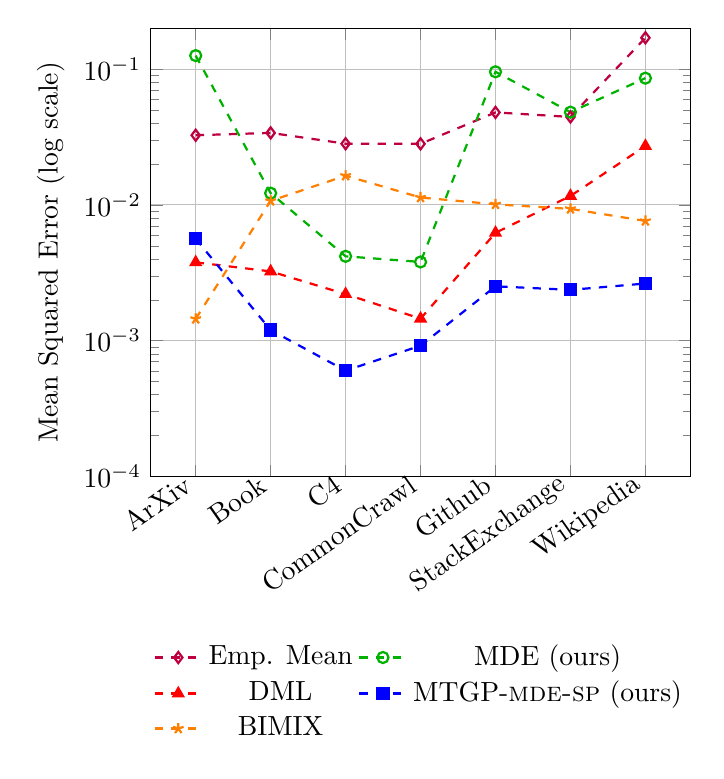
\begin{tikzpicture}
    \begin{axis}[
      ylabel={Mean Squared Error (log scale)},
      ymode=log,
      symbolic x coords={ArXiv,Book,C4,CommonCrawl,Github,StackExchange,Wikipedia},
      xtick=data,
      ymin=0.0001,
      ymax=0.2,
      grid=major,
      legend style={at={(0.5,-0.35)}, anchor=north, legend columns=2, draw=none}, % Modified to 2 columns
      x tick label style={rotate=35, anchor=east},
      mark options={solid},
    %   width=0.95\textwidth, % Make the plot wider
    %   height=0.6\textwidth, % Adjust the height to keep aspect ratio
    ]

      % emp. mean
      \addplot[dashed, mark=diamond, color=purple, thick] coordinates {
        (ArXiv,0.03258848761214498) 
        (Book,0.033901799466678983) 
        (C4,0.028237080166221618) 
        (CommonCrawl,0.028170427516745984) 
        (Github,0.04799648997394152) 
        (StackExchange,0.04444072752490156) 
        (Wikipedia,0.16998068744909084)
      };
      \addlegendentry{Emp. Mean}

      % mde
      \addplot[dashed, mark=o, color=green!70!black, thick] coordinates { % Darker green
        (ArXiv,0.12569990165231987) 
        (Book,0.012200067712023305) 
        (C4,0.004183705236557251) 
        (CommonCrawl,0.0038020182635709896) 
        (Github,0.09553608975123355) 
        (StackExchange,0.048190113535861154) 
        (Wikipedia,0.08576905332796389)
      };
      \addlegendentry{MDE (ours)}

      % dml
      \addplot[dashed, mark=triangle*, color=red, thick] coordinates {
        (ArXiv,0.0037785496210790935) 
        (Book,0.0032396400943874803) 
        (C4,0.0022037963338795985) 
        (CommonCrawl,0.0014545846122193365) 
        (Github,0.006231348171967968) 
        (StackExchange,0.01163995357956378) 
        (Wikipedia,0.027135803524510626)
      };
      \addlegendentry{DML}

      % mtgp_mde
      \addplot[dashed, mark=square*, color=blue, thick] coordinates {
        (ArXiv,0.005638437945592803) 
        (Book,0.001197677572446236) 
        (C4,0.0006021703300710033) 
        (CommonCrawl,0.0009188736749797932) 
        (Github,0.0025156553673455454) 
        (StackExchange,0.002369188450940196) 
        (Wikipedia,0.0026375685939519487)
      };
      \addlegendentry{MTGP-\textsc{mde-sp} (ours)}

      % bimix
      \addplot[dashed, mark=star, color=orange, thick] coordinates {
        (ArXiv,0.0014483220708567256) 
        (Book,0.010711812127249159) 
        (C4,0.01641659212707495) 
        (CommonCrawl,0.01133554534292917) 
        (Github,0.010100280035751018) 
        (StackExchange,0.00934835484835737) 
        (Wikipedia,0.0076224179394367726)
      };
      \addlegendentry{BIMIX}

    \end{axis}
  \end{tikzpicture}
  }
  \caption{Per-domain mean loss squared error for SlimPajama validation domains.}
  \label{fig:280M_to_280M_train_only_loss_error_per_domain_sxs}
\end{figure}








\subsubsection*{Extrapolation to mixtures of the same scale}

In the first set of experiments, we aim to assess the ability of different methods to predict validation losses and loss aggregates for new mixtures $\lambda$, given a training set of measurements for models of the same size and number of training steps.



We look at per-validation domain performance, as well as the performance corresponding to multiple loss aggregators ---
 \textsc{avg-sp}: Average loss on the seven SlimPajama validation datasets,% (equally weighted),
     %drawn from the training domains
    which has been a common optimization target used by baselines including DoGe and DML; 
    % Note this is the generalization loss estimate optimized by DoGe and DML;
    \textsc{avg-et}: Average loss on the eleven validation end task domains detailed in Section~\ref{sec:data};
    %(equally weighted);
    \textsc{avg-et+sp}: Average loss across all 18 validation domains -- the union of SlimPajama and end task validation datasets.% 


We evaluate regression methods using squared error between predicted and true loss values, along with Spearman's rank correlation. A training set of 25 mixtures and a test set of 48 distinct mixtures, each with 280M-sized models trained for 10K steps (5B tokens), are used for comparison. Table~\ref{tab:regressors_sxs} reports mean squared error and Spearman’s rank correlation for \textsc{avg-sp} and \textsc{avg-et+sp} aggregated losses. Figure~\ref{fig:280M_to_280M_train_only_loss_error_per_domain_sxs} shows squared error for each individual SlimPajama validation domain.  The reported results are averages from 5 training runs for each method, with a different sampled training set of mixtures for each run.

For the regressors using MDE features, we denote with e.g. MTGP-\textsc{MDE-sp} models that use the MDE features only from the 7 \textsc{sp} domains, and also predict the losses only on those domains. In Table~\ref{tab:regressors_sxs}, the regressors using MDE use only the \textsc{sp} domain features for the results in the first two columns, and all 18 MDE features for the results in the second two columns. 

We note that: (\textit{i}) As a standalone predictor, MDE performs no better than the empirical mean baseline in loss prediction for \textsc{avg-sp}, while substantially outperforming that baseline for \textsc{avg-et+sp}. (\textit{ii}) As a standalone ranker, MDE's performance is very respectable and close to that of the best regressors which use 3x more trained proxy models. (\textit{iii}) MDE as a source of features brings large improvements in MSE and Spearman's, across multiple regression model families (Linear, MTGP, GBM), (e.g. improvement from 0.65 to 0.95 for linear regressors),  substantially improving over prior state-of-the-art regressors, while using equivalent computational resources. Note that while we only report the mean and not the confidence intervals for each predictor in the table, we verified the gains are statistically significant. In Appendix~\ref{sec:model_merge} we consider alternate ways to approximate data mixture losses using trained experts, showing MDE achieves superior performance.
    
   







\subsubsection*{Extrapolating to larger scale models}

Our ultimate goal is to compare and optimize mixtures according to the performance corresponding to the largest models, trained for a maximum token budget (here 1B models and 100B tokens). While \textsc{RegMix}~\citep{regmix} found that very small models trained over relatively few tokens (1M model size and 1B tokens) are sufficient as proxies for learning to rank much more scaled versions, we find that the approximation quality is dependent on the choice of generalization loss estimate we aim to optimize.  To understand this, we train proxy  models of different sizes corresponding to the same set of $55$ data mixtures $\lambda$. The proxies are of sizes $70$M, $150$M, $280$M, and $510$M, and are trained to a token horizon of up to 50K steps (25B tokens). We then see whether the ranking of the mixtures at the largest configuration ($510$M, $50$K steps) can be predicted through the true losses of proxies of different scales for the same mixtures.\footnote{Note that our model sizes are total parameters and the number of non-embedding ones is smaller, e.g. 2.6M for the 70M model and 85M for the 280M model, see Appendix~\ref{sec:appendix_lms}.}


Figure~\ref{fig:proxyranking} shows that, as \textsc{RegMix} observed, ranking according to a single training domain, SlimPajama {\small{CommonCrawl}}, is well predicted by all proxy models, with a small difference between 70M and 280M models and a small improvement with the number of training steps (dashed lines). On the other hand, for a harder ranking metric, which requires mixtures to be ordered correctly simultaneously according to the three aggregate losses \textsc{avg-sp}, \textsc{avg-et}, and \textsc{avg-et+sp}, 70M  models and ones trained to less than 6K steps are substantially less accurate proxies. We thus choose to use 280M models trained to 10K steps as proxies for optimizing 1B-sized models trained to 200K steps, as a tradeoff between accuracy and efficiency.



\begin{figure}[t]
  \centering
  \begin{minipage}{0.48\textwidth}
    \centering
    \scalebox{0.75}{ 
      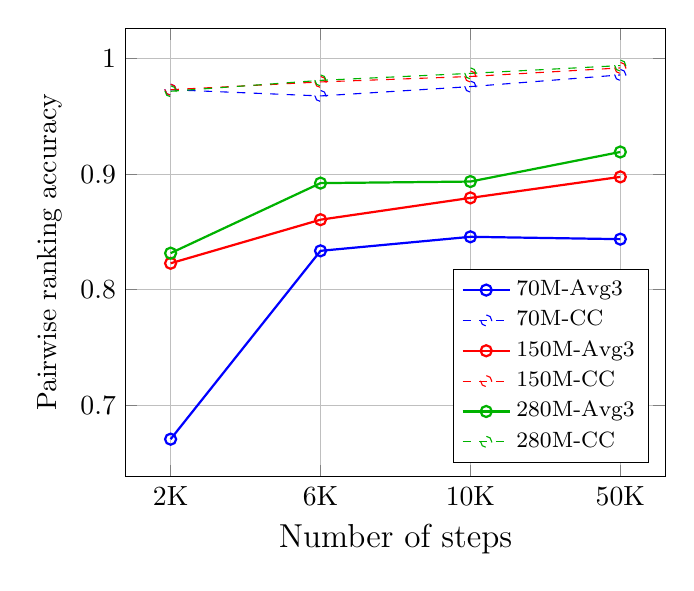
\begin{tikzpicture}
        \begin{axis}[
          xlabel=Number of steps,
          xlabel style={font=\large},
          ylabel=Pairwise ranking accuracy,
          grid=major,
          legend pos=south east,
          legend cell align=left,
          legend style={font=\footnotesize},
          title style={font=\large},
          xtick={1,2,3,4},
          xticklabels={2K, 6K, 10K, 50K}
        ]
        
        \addplot[thick, color=blue, mark=o] coordinates {
          (1, 0.6707070707070707)
          (2, 0.8336700336700337)
          (3, 0.8457912457912458)
          (4, 0.8437710437710437)
        };
        \addlegendentry{70M-Avg3}

        \addplot[dashed, color=blue, mark=o] coordinates {
          (1, 0.9730639730639731)
          (2, 0.9676767676767677)
          (3, 0.9757575757575757)
          (4, 0.9858585858585859)
        };
        \addlegendentry{70M-CC}

        \addplot[thick, color=red, mark=o] coordinates {
          (1, 0.8228956228956229)
          (2, 0.8606060606060606)
          (3, 0.8794612794612795)
          (4, 0.8976430976430977)
        };
        \addlegendentry{150M-Avg3}

        \addplot[dashed, color=red, mark=o] coordinates {
          (1, 0.9730639730639731)
          (2, 0.9797979797979798)
          (3, 0.9845117845117846)
          (4, 0.9919191919191919)
        };
        \addlegendentry{150M-CC}

        \addplot[thick, color=green!70!black, mark=o] coordinates {
          (1, 0.8316498316498316)
          (2, 0.8922558922558923)
          (3, 0.8936026936026936)
          (4, 0.9191919191919192)
        };
        \addlegendentry{280M-Avg3}

        \addplot[dashed, color=green!70!black, mark=o] coordinates {
          (1, 0.9717171717171718)
          (2, 0.9811447811447811)
          (3, 0.9872053872053872)
          (4, 0.9939393939393939)
        };
        \addlegendentry{280M-CC}
        \end{axis}
      \end{tikzpicture}
    }
    \caption{Pairwise ranking accuracy of 55 data mixtures (510M models trained to 50K steps) based on proxies of different size and number of training steps.}
    \label{fig:proxyranking}
  \end{minipage}
\end{figure}



 
\subsubsection*{Learning curve: impact of number of training mixtures}

We analyze how ranking performance scales with the number of training examples. Figure~\ref{fig:learning_curve_280M_510M} illustrates the learning curve for Spearman's rank correlation of the average loss (\textsc{avg-sp}). Sets of 280M-parameter proxy models, trained for 10K steps are used to predict the ranking order of the average domain loss for larger 510M-parameter models from unseen data mixtures, trained for 50K steps.

In the low-data regime,  MDE consistently outperforms all other models. However, as more training examples become available, MTGP-\textsc{mde-sp} and \textsc{Linear}-\textsc{mde-sp} steadily improve, eventually surpassing MDE to achieve the best performance. For ranking according to the \textsc{avg-sp} loss, we observe diminishing returns beyond 25 training examples, suggesting a saturation point in the benefits of additional data.



\begin{figure}[t]
  \centering
   \begin{minipage}{0.5\textwidth}
        \centering
 \scalebox{.75}{
  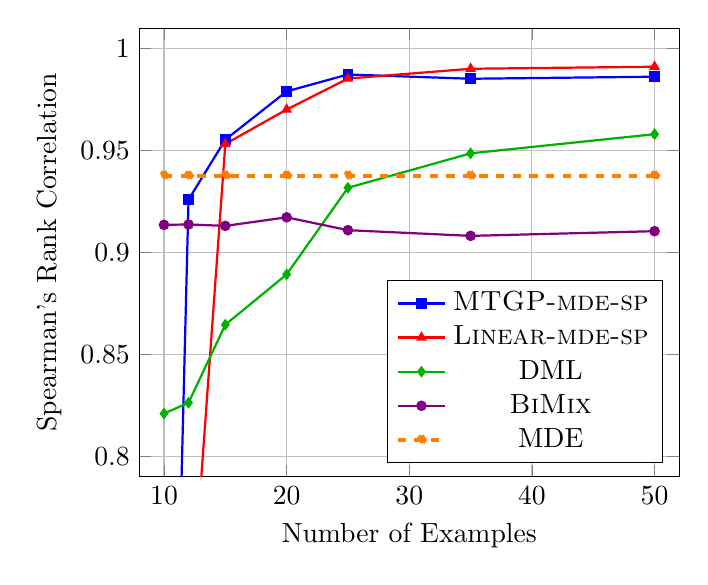
\begin{tikzpicture}
    \begin{axis}[
      xlabel={Number of Examples},
      ylabel={Spearman's Rank Correlation},
      legend pos=south east,
      grid=major,
      enlargelimits=0.05,
      ymin=0.8, ymax=1,
      xmin=10, xmax=50,
      mark size=1.5pt,
      every mark/.append style={solid},
    ]
    \addplot+[mark=square*, thick, color=blue] coordinates {(10, 0.4461) (12, 0.9259) (15, 0.9553) (20, 0.9790) (25, 0.9873) (35, 0.9852) (50, 0.9862)};
    \addlegendentry{\textsc{MTGP-mde-sp}}

    \addplot+[mark=triangle*, thick, color=red] coordinates {(10, 0.6358) (12, 0.7029) (15, 0.9532) (20, 0.9701) (25, 0.9853) (35, 0.9901) (50, 0.9911)};
    \addlegendentry{\textsc{Linear-mde-sp}}

    \addplot+[mark=diamond*, thick, color=green!70!black] coordinates {(10, 0.8209) (12, 0.8262) (15, 0.8645) (20, 0.8892) (25, 0.9317) (35, 0.9486) (50, 0.9580)};
    \addlegendentry{DML}

    \addplot+[mark=*, thick, color=violet] coordinates {(10, 0.9135) (12, 0.9137) (15, 0.9130) (20, 0.9172) (25, 0.9109) (35, 0.9081) (50, 0.9104)};
    \addlegendentry{\textsc{BiMix}}

    \addplot+[dashed, ultra thick, color=orange] coordinates {(10, 0.9376) (12, 0.9376) (15, 0.9376) (20, 0.9376) (25, 0.9376) (35, 0.9376) (50, 0.9376)};
    \addlegendentry{MDE}
    \end{axis}
  \end{tikzpicture}
  }
  \end{minipage}
  \caption{Spearman's rank correlation of \textsc{sp} validation domains as a function of number of training mixtures. }
  %Ranking 510M models based on training examples from 280M proxies.
  \label{fig:learning_curve_280M_510M}
\end{figure}

\subsection{Correlation between validation loss and downstream task accuracy}
\label{sec:correlationdownstream}

\begin{table}[t]
    \centering
    \begin{small}
    \begin{sc}
    \scalebox{0.8}{
    \begin{tabular}{@{\hspace{2pt}}l@{\hspace{4pt}}|@{\hspace{4pt}}c@{\hspace{4pt}}c@{\hspace{4pt}}|c@{\hspace{4pt}}c@{\hspace{4pt}}c@{\hspace{2pt}}}
    \toprule
    \multirow{2}{*}{Val. Task} & \multicolumn{2}{c|}{Val. Tasks} & \multicolumn{3}{c}{Downstream Tasks} \\
     & Self & Avg. & Gen. & Rank. & All \\
    \midrule
    ARC-C & $0.452$ & $0.771$ & $0.613$ & $0.846$ & $0.845$  \\
    ARC-E & $0.903$ & $0.761$ & $0.608$ & $0.845$ & $0.840$ \\
    OpenBookQA & $0.862$ & $0.785$ & $0.626$ & $0.840$ & $0.846$ \\
    MultiRC & $0.245$ & $0.698$ & $0.653$ & $0.728$ & $0.796$ \\
    Average-ET & --- &  $0.772$ & $0.630$ & $0.833$  & $0.844$ \\
    \midrule
     ArXiv & --- &  \hspace{-0.3cm}$-0.248$ & ~\hspace{-0.28cm}$-0.198$ & ~\hspace{-0.3cm}$-0.166$ & \hspace{-0.3cm}$-0.233$ \\
     Book & --- &  $0.514$ & $0.442$ & $0.603$ & $0.571$ \\
     C4 & --- &  $0.725$ & $0.508$ & $0.821$ & $0.767$ \\
     CommonCrawl & --- &  $0.673$ & $0.636$ & $0.609$ & $0.740$ \\
      Github & --- &  \hspace{-0.3cm}$-0.299$ & ~\hspace{-0.28cm}$-0.256$ & ~\hspace{-0.3cm}$-0.306$ & \hspace{-0.3cm}$-0.336$ \\
     StackExchange & --- &  \hspace{-0.3cm}$-0.107$ & ~\hspace{-0.28cm}$-0.039$ & ~\hspace{-0.3cm}$-0.120$ & \hspace{-0.3cm}$-0.093$ \\
     Wikipedia & --- &  $0.146$ & $0.013$ & $0.093$ & $0.045$ \\
    Average-SP & --- &  $0.320$ & $0.189$ & $0.330$ & $0.282$ \\
    \bottomrule
    \end{tabular}
    }
    \end{sc}
    \end{small}
    \caption{Spearman's rank correlation between validation tasks' loss and accuracy metrics, considering the same task ({\sc Self}), the average accuracy across all validation end tasks ({\sc Avg.}), and metrics for downstream test tasks: average on the generation ({\sc Gen.}),  ranking  ({\sc Rank.}), and all test tasks ({\sc All}).}
    \label{tab:end-task-correlation}
\end{table}


Section~\ref{sec:results-loss-prediction} shows that our methods produce more accurate validation loss prediction results than prior methods.
Can such improvement help guide us towards finding mixture weights that improve on downstream evaluations?
In downstream tasks, models are usually evaluated based on generation or ranking accuracies instead of cross-entropy loss.
Additionally, capable models should generalize beyond tasks seen during development and should perform well on unseen tasks.
To understand the potential impact of the choice of using \textsc{avg-et} as a mixture weight optimization objective, we conduct a study comparing end task validation loss and test accuracies using 510M parameter models trained up to 50K steps.
As observed in Table~\ref{tab:end-task-correlation}, there is a strong correlation\footnote{Correlations are negative because a lower language modeling loss typically corresponds to better end task evaluation results. In Table~\ref{tab:end-task-correlation}, we show the absolute values for readability.} between validation tasks' language modeling loss and model performance on the downstream test tasks.
In contrast, the average SP domains' validation losses (last row) show much lower correlation with end task evaluation results. From the SP domains, C4 and CommonCrawl which have the highest correlation with downstream task accuracy.



\subsection{Results with optimized data mixtures}

Based on our study with models in the range of 70M to 510M parameters, we choose to optimize training mixtures using well-performing regressors for each objective of interest, from 280M-sized proxies. We optimize mixtures for three different criteria: (\textit{i}) \textsc{avg-sp} the average loss on SlimPajama domains, (\textit{ii}) \textsc{avg-et}, the average loss on  end task validation domains, and (\textit{iii}) \textsc{avg-sp} + \textsc{avg-et}, also called \textsc{avg-all}, the sum of the two averages. Much prior work has focused on optimizing \textsc{avg-sp} or the loss on a single domain. Section~\ref{sec:correlationdownstream} shows \textsc{avg-et} correlates better with downstream accuracy, though a small set of validation tasks may not be sufficient to cover all requisite skills for LM generalization. Thus, we consider the combination of the unsupervised loss (\textsc{avg-sp}) with the end-task aware loss (\textsc{avg-et}).

To optimize the mixtures, we trained regressor models using 25 mixture examples (including the 7 experts), each of size 280M trained to 10K steps. The optimized models for the three criteria are denoted as \textsc{MTGP-mde-sp}, \textsc{Linear-mde-et}, and \textsc{Linear-mde-all} in the tables and figures. Their corresponding mixture weights are given in Appendix~\ref{sec:appendix_results}.


\begin{table*}[htbp!]
  \centering
  \begin{small}
  \begin{sc}
  \scalebox{0.75}{
  \begin{tabular}{@{\hspace{4pt}}l@{\hspace{4pt}}l|c@{\hspace{10pt}}c@{\hspace{8pt}}c@{\hspace{4pt}}c@{\hspace{4pt}}c|c@{\hspace{4pt}}c@{\hspace{4pt}}c@{\hspace{4pt}}c@{\hspace{4pt}}c|c}
  \toprule
  & \multirow{2}{*}{Model} & \multicolumn{5}{c|}{Generation Tasks} & \multicolumn{5}{c|}{Ranking Tasks} & \multirow{2}{*}{Average ($\uparrow$)} \\
    &  & WQ & NQ & \scriptsize{SQuAD} & \scriptsize{TriviaQA} & \scriptsize{LAMBADA} & COPA & PiQA & WiC & \scriptsize{WinoGrande} & \scriptsize{HellaSwag} & \\
  \midrule
    & Uniform & $4.4$  &  $2.4$  &  $35.8$  &  $10.9$  &  ${21.9}$  &  $70.0$  &  $67.9$  &  $49.1$  &  $54.2$  &  $42.3$  &  $35.9$ \\
    & SlimPajama & $\mathbf{6.9}$  &  $\mathbf{3.9}$  &  $37.0$  &  ${15.7}$  &  $18.9$  &  $71.3$  &  $67.2$  &  $49.5$  &  $54.7$  &  $45.3$  &  $37.0$ \\
    & DoGE (124M) & $5.2$  &  $2.3$  &  $33.5$  &  $10.0$  &  $19.9$  &  $70.0$  &  $68.4$  &  $48.1$  &  $54.0$  &  $43.1$  &  $35.4$ \\
    & DoReMi (124M) & $5.1$  &  $2.8$  &  $37.1$  &  $13.6$  &  $21.7$  &  $71.7$  &  $66.4$  &  $48.8$  &  $54.5$  &  $42.3$  &  $36.4$ \\
    \multirow{-5}{*}{\rotatebox[origin=c]{90}{Baselines}}
    & DML & $4.1$  &  $1.9$  &  $34.4$  &  $~~9.1$  &  $15.5$  &  $71.7$  &  $68.1$  &  $\mathbf{50.9}$  &  $54.0$  &  $42.9$  &  $35.3$ \\
  \midrule
    & \textsc{MTGP-mde-sp} & $4.0$  &  $2.4$  &  $34.2$  &  $9.4$  &  $19.6$  &  $68.7$  &  $67.6$  &  $50.4$  &  $52.8$  &  $43.0$  &  $35.2$ \\
    \multirow{-2}{*}{\rotatebox[origin=c]{90}{\scriptsize{Ours}}}
   % & MTGP-MDE-Task & $6.2$  &  $3.3$  &  $\mathbf{39.1}$  &  $14.7$  &  $21.4$  &  $\mathbf{73.7}$  &  $\mathbf{69.7}$  &  $48.7$  &  $\mathbf{57.1}$  &  $\mathbf{46.7}$  &  $\mathbf{38.0}$ \\
 & \textsc{Linear-mde-et} & $6.4$ & $3.5$ & $34.7$ & $\mathbf{17.6}$ & $22.1$ & $\mathbf{75.3}$ & $69.3$ & $49.3$ &  $\mathbf{55.7}$ & $47.6$ & $38.2$ \\
 & \textsc{Linear-mde-all} & $6.1$ & $3.1$ & $\mathbf{37.2}$ & $14.7$ & $\mathbf{24.1}$ & $73.3$ & $\mathbf{70.4}$ & $50.4$ &  $\mathbf{55.7}$ & $\mathbf{47.7}$ & $\mathbf{38.3}$ \\
  \bottomrule
  \end{tabular}
  }
  \end{sc}
  \end{small}
  \caption{Downstream model performance on $5$ prediction tasks and $5$ ranking tasks. Results are averaged across $0$-shot, $1$-shot, and $5$-shot performances.  For generation tasks, we report exact match (EM) accuracies (\%), and for ranking tasks, we report accuracies (\%).  All models are 1B parameter models trained for 200K steps.}
  \label{tab:downstream-results-main}
\end{table*}


%%%backup

\begin{figure}[]
\centering
\begin{minipage}{\columnwidth}

\scalebox{0.55}{

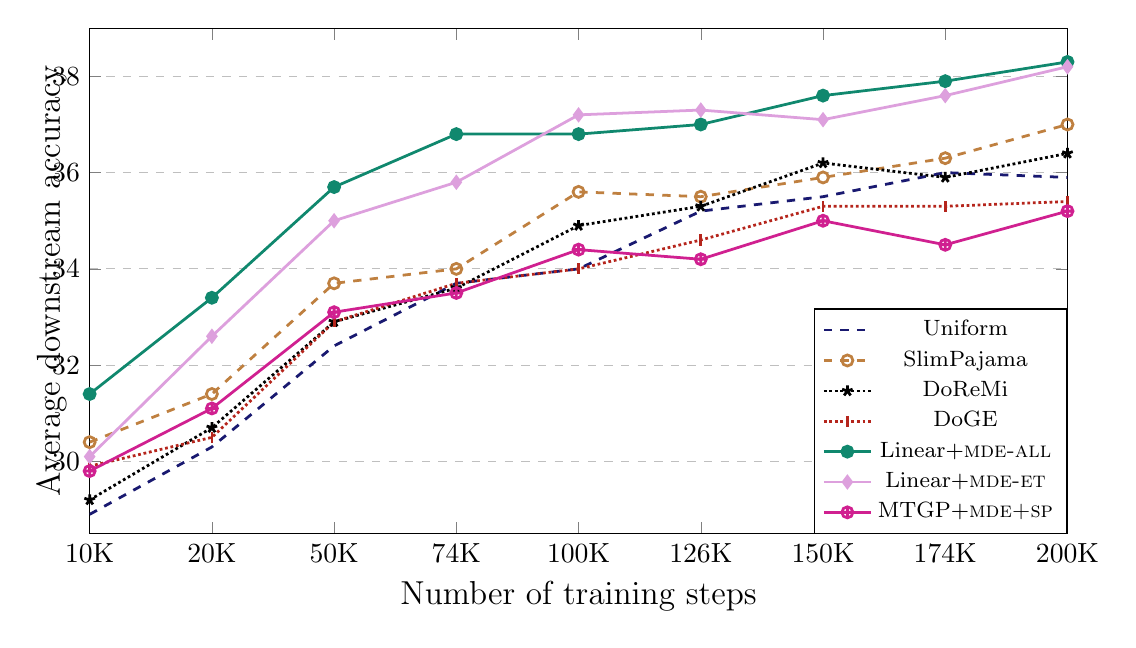
\begin{tikzpicture}
    \begin{axis}[
        xlabel={Number of training steps},
        xlabel style={font=\large},
        ylabel={Average downstream accuracy},
        ylabel style={yshift=-12pt, font=\large},
        legend pos=south east,
        ymin=28.5, ymax=39.0,
        xmin=1,xmax=9,
        legend style={at={(1,0)}, anchor=south east},
        ymajorgrids=true,
        grid style=dashed,
        width=14cm,
        height=8cm,
        %xmode=log,
        xtick={1,2,3,4,5,6,7,8,9}, % Positions for the x-ticks
        xticklabels={10K, 20K, 50K, 74K, 100K, 126K,150K,174K,200K}, % Custom x-tick labels
        legend style={font=\footnotesize}, % Make legend text smaller
    ]

        \addplot[color=MidnightBlue, line width=1pt, dashed, mark options=solid] coordinates {(1, 28.9) (2, 30.3) (3, 32.4) (4, 33.7) (5, 34.0) (6, 35.2) (7, 35.5) (8, 36.0) (9, 35.9)};
        \addlegendentry{Uniform}

        \addplot[color=brown, mark=o, line width=1pt, dashed, mark options=solid] coordinates {(1, 30.4) (2, 31.4) (3, 33.7) (4, 34.0) (5, 35.6) (6, 35.5) (7, 35.9) (8, 36.3) (9, 37.0) };
        \addlegendentry{SlimPajama}

        \addplot[color=black, mark=star, line width=1pt, densely dotted, mark options=solid] coordinates {(1, 29.2) (2, 30.7) (3, 32.9) (4, 33.6) (5, 34.9) (6, 35.3) (7, 36.2) (8, 35.9) (9, 36.4)};
        \addlegendentry{DoReMi}

        \addplot[color=BrickRed, mark=|, line width=1pt, densely dotted, mark options=solid] coordinates {(1, 29.9) (2, 30.5) (3, 32.9) (4, 33.7) (5, 34.0) (6, 34.6) (7, 35.3) (8, 35.3) (9, 35.4) };
        \addlegendentry{DoGE}

        \addplot[color=PineGreen, mark=*, line width=1pt] coordinates {(1, 31.4) (2, 33.4) (3, 35.7) (4, 36.8) (5, 36.8) (6, 37.0) (7, 37.6) (8, 37.9) (9, 38.3)};
        \addlegendentry{Linear+\textsc{mde-all}}

        \addplot[color=Plum, mark=diamond*, line width=1pt] coordinates {(1, 30.1) (2, 32.6) (3, 35.0) (4, 35.8) (5, 37.2) (6, 37.3) (7, 37.1) (8, 37.6) (9, 38.2)};
        \addlegendentry{Linear+\textsc{mde-et}}

        \addplot[color=VioletRed, mark=oplus, line width=1pt] coordinates {(1, 29.8) (2, 31.1) (3, 33.1) (4, 33.5) (5, 34.4) (6, 34.2) (7, 35.0) (8, 34.5) (9, 35.2)};
        \addlegendentry{MTGP+\textsc{mde+sp}}

        \draw [decorate,decoration={brace,amplitude=5pt},yshift=0pt,xshift=250pt]
      (7,25) -- (7,32) node [midway,left,xshift=-5pt] {Prior work};

        \draw [decorate,decoration={brace,amplitude=5pt},yshift=0pt,xshift=250pt]
      (7,5) -- (7,18) node [midway,left,xshift=-5pt] {Ours};
        %\node at (1.2,22) {Ours};

    \end{axis}
\end{tikzpicture}
}
\end{minipage}
\caption{Downstream task accuracy (average over 0-shot,1-shot, and 5-shot formulations over a suite of generation and ranking tasks) for 1B models optimized through our methods using MDE versus prior work.}
\label{fig:downstream}
\end{figure}


 %\textcolor{red}{Note to reviewers: these numbers will be updated with Linear+MDE models and optimization from 25 models at 10K steps instead of 39 models at 50K steps.}

In Table~\ref{loss-1b-training} we see that the mixture optimized with MTGP-\textsc{mde} for \textsc{avg-sp} loss leads to a full-scale model that achieves the best \textsc{avg-sp} generalization loss compared to prior work that optimized the same loss ({\doge} and DML), and other baselines. In that table and other comparisons in this section, we use the mixture weights optimized in prior work directly from the corresponding papers, and train 1B models with those weights for comparison.  For {\doge} and {\doremi}, we used the mixture weights reported in \citet{DOGE}, optimized from their 124M proxies which are similar in scale to our 280M proxies in the number of non-embedding parameters. We note that differences in tokenization and other hyper-parameters could have results in different optimized weights if we had applied the prior work's methods on our data to derive the mixture weights.

In Table~\ref{loss-1b-withendtask}, we additionally include models optimized for the losses of the two other end-task related criteria.\footnote{These optimized weights included 0 values for some domains and we smoothed the solutions $\hat{\lambda} = .99 \lambda_{\mbox{opt}} + .01 \mathbf{uniform}$.} As we see, our approaches lead to successful optimization of the desired generalization losses for the full size models.
%on SplimPajama and end-task domains (\textsc{avg-sp}+\textsc{avg-ET}), while still reporting the average \textsc{avg-sp} from the prior table.
%We see that MTGP-MDE-{\tiny{TASK}} achieves better tuning task and overall average loss for the fully trained 1B models. 






\begin{table}[t]
\begin{center}
\begin{small}
\begin{sc}
\scalebox{0.6}{
\begin{tabular}{l@{}rrrrrrr}
\toprule
 & Uniform  & SlimPajama  & DoGE & DoReMI & DML &  \textsc{MTGP-mde-sp} \\
\midrule
ArXiv  &  4.90 & 5.41 & 5.06 & 5.45 & 4.64 & 5.13 \\
Book  &  14.77 & 15.28 & 15.76 & 15.44 & 15.40 & 15.12 \\
C4  &  17.62 & 15.72 & 16.41 & 17.08 & 17.00 & 16.93 \\
CommCrawl  &  14.43 & 12.52 & 13.78 & 13.22 & 14.52 & 14.25 \\
Github  &  2.59 & 2.89 & 2.71 & 2.77 & 2.58 & 2.64 \\
StackExch.  &  5.33 & 6.12 & 5.26 & 5.65 & 5.33 & 5.33 \\
Wikipedia  &  8.89 & 10.67 & 8.70 & 8.09 & 13.02 & 8.24 \\
\midrule
Average   &  8.085 & 8.449 & 8.072 & 8.156 & 8.482 & \textbf{8.038} \\

\bottomrule
\end{tabular}
}
\end{sc}
\end{small}
\caption{Generalization on validation \textsc{sp} domains for 1B parameter models trained for 100B tokens with mixtures optimized according to different methods  over the \textsc{sp} domains. We compare Baselines (uniform and proportional to size), DoGE(124M), DoReMI (124M), to the mixture derived by \textsc{MTGP-mde-sp}. Per-domain and average (exponentiatated average loss) perplexity.} % results are at 200K steps
\label{loss-1b-training}

\end{center}
\end{table}





\begin{table}[]
\vskip 0.15in
\begin{center}
\begin{small}
\begin{sc}
\scalebox{0.48}{
\begin{tabular}{l@{}rrrrrrrrr}
\toprule
 & \textsc{Uniform}  & \textsc{SlimPJ}  & \textsc{DoGE} & \textsc{DoReMI}  & DML &  \textsc{MTGP-mde-sp} & \textsc{Lin-mde-et} & \textsc{Lin-mde-all} \\ & & & & & & \textsc{(OURS)} & \textsc{(OURS)} & \textsc{(OURS)}\\
\midrule
%ARC-c  &  19.93 & 17.81 & 19.45 & 19.37 & 19.54 & 19.16 & 17.86 \\
ARC-c  &  19.93 & 17.81 & 19.45 & 19.37 & 19.54 & 20.02 & \textbf{16.92} & 17.72 \\
%ARC-e  &  20.86 & 18.57 & 20.52 & 20.33 & 20.66 & 20.07 & 18.57 \\
ARC-e  &  20.86 & 18.57 & 20.52 & 20.33 & 20.66 &  21.17 & \textbf{17.55}  & 18.45 \\
% ObQA  &  48.45 & 44.99 & 48.20 & 47.60 & 48.09 & 48.09 & 44.03 \\
ObQA  &  48.45 & 44.99 & 48.20 & 47.60 & 48.09 &  48.00 & \textbf{43.78}  &  44.17\\
%MultiRC  &  10.44 & 9.80 & 10.40 & 10.21 & 10.59 & 10.37 & 9.78 \\
MultiRC  &  10.44 & 9.80 & 10.40 & 10.21 & 10.59 & 10.36 & \textbf{9.56} &  9.67 \\
\midrule
%Avg. SP  &  8.085 & 8.449 & 8.072 & 8.156 & 8.482 & \textbf{8.038} & 8.400  \\
Avg. SP  &  8.08 & 8.45 & 8.07 & 8.16 & 8.48 & \textbf{8.04} & 10.44  & 9.26  \\
%Avg. task     &  22.860 & 20.807 & 22.557 & 22.322 & 22.690 & 22.303 & \textbf{20.692} \\
Avg. ET     &  22.86 & 20.81 & 22.56 & 22.32 & 22.69 & 22.89 & \textbf{19.96} & 20.59 & \\
\bottomrule
\end{tabular}
}
\caption{{Generalization on end task validation domains for 1B parameter models trained for 100B tokens. Our model mixtures are optimized based on different generalization criteria, \textsc{avg-sp}, \textsc{avg-et}, and \textsc{avg-all}. We compare mixtures from baselines and prior work to mixtures derived by our methods \textsc{MTGP-mde-sp}, \textsc{Linear-mde-et}, and \textsc{Linear-mde-all}. We report per-domain group and average perplexity.} }
\label{loss-1b-withendtask}
\end{sc}
\end{small}
\end{center}
\vskip -0.1in
\end{table}





\subsection{Downstream task few-shot prediction}



We compare model performance on downstream tasks in Table~\ref{tab:downstream-results-main} with learning curves in Figure~\ref{fig:downstream}.
We observe that the token-proportional SlimPajama baseline is a strong baseline as it outperforms the uniform baseline and other baseline from prior work including {\doge}, {\doremi}, and DML \cite{dml}.
While our model that is optimized for the  \textsc{avg-sp} loss has relatively low average accuracy, our model variants that are optimized taking into account validation end tasks \textsc{Linear-mde-et} and \textsc{Linear-mde-all} outperform all baselines and models from prior work.








